% Options for packages loaded elsewhere
% Options for packages loaded elsewhere
\PassOptionsToPackage{unicode}{hyperref}
\PassOptionsToPackage{hyphens}{url}
\PassOptionsToPackage{dvipsnames,svgnames,x11names}{xcolor}
%
\documentclass[
  letterpaper,
  DIV=11,
  numbers=noendperiod]{scrartcl}
\usepackage{xcolor}
\usepackage{amsmath,amssymb}
\setcounter{secnumdepth}{-\maxdimen} % remove section numbering
\usepackage{iftex}
\ifPDFTeX
  \usepackage[T1]{fontenc}
  \usepackage[utf8]{inputenc}
  \usepackage{textcomp} % provide euro and other symbols
\else % if luatex or xetex
  \usepackage{unicode-math} % this also loads fontspec
  \defaultfontfeatures{Scale=MatchLowercase}
  \defaultfontfeatures[\rmfamily]{Ligatures=TeX,Scale=1}
\fi
\usepackage{lmodern}
\ifPDFTeX\else
  % xetex/luatex font selection
\fi
% Use upquote if available, for straight quotes in verbatim environments
\IfFileExists{upquote.sty}{\usepackage{upquote}}{}
\IfFileExists{microtype.sty}{% use microtype if available
  \usepackage[]{microtype}
  \UseMicrotypeSet[protrusion]{basicmath} % disable protrusion for tt fonts
}{}
\makeatletter
\@ifundefined{KOMAClassName}{% if non-KOMA class
  \IfFileExists{parskip.sty}{%
    \usepackage{parskip}
  }{% else
    \setlength{\parindent}{0pt}
    \setlength{\parskip}{6pt plus 2pt minus 1pt}}
}{% if KOMA class
  \KOMAoptions{parskip=half}}
\makeatother
% Make \paragraph and \subparagraph free-standing
\makeatletter
\ifx\paragraph\undefined\else
  \let\oldparagraph\paragraph
  \renewcommand{\paragraph}{
    \@ifstar
      \xxxParagraphStar
      \xxxParagraphNoStar
  }
  \newcommand{\xxxParagraphStar}[1]{\oldparagraph*{#1}\mbox{}}
  \newcommand{\xxxParagraphNoStar}[1]{\oldparagraph{#1}\mbox{}}
\fi
\ifx\subparagraph\undefined\else
  \let\oldsubparagraph\subparagraph
  \renewcommand{\subparagraph}{
    \@ifstar
      \xxxSubParagraphStar
      \xxxSubParagraphNoStar
  }
  \newcommand{\xxxSubParagraphStar}[1]{\oldsubparagraph*{#1}\mbox{}}
  \newcommand{\xxxSubParagraphNoStar}[1]{\oldsubparagraph{#1}\mbox{}}
\fi
\makeatother

\usepackage{color}
\usepackage{fancyvrb}
\newcommand{\VerbBar}{|}
\newcommand{\VERB}{\Verb[commandchars=\\\{\}]}
\DefineVerbatimEnvironment{Highlighting}{Verbatim}{commandchars=\\\{\}}
% Add ',fontsize=\small' for more characters per line
\usepackage{framed}
\definecolor{shadecolor}{RGB}{241,243,245}
\newenvironment{Shaded}{\begin{snugshade}}{\end{snugshade}}
\newcommand{\AlertTok}[1]{\textcolor[rgb]{0.68,0.00,0.00}{#1}}
\newcommand{\AnnotationTok}[1]{\textcolor[rgb]{0.37,0.37,0.37}{#1}}
\newcommand{\AttributeTok}[1]{\textcolor[rgb]{0.40,0.45,0.13}{#1}}
\newcommand{\BaseNTok}[1]{\textcolor[rgb]{0.68,0.00,0.00}{#1}}
\newcommand{\BuiltInTok}[1]{\textcolor[rgb]{0.00,0.23,0.31}{#1}}
\newcommand{\CharTok}[1]{\textcolor[rgb]{0.13,0.47,0.30}{#1}}
\newcommand{\CommentTok}[1]{\textcolor[rgb]{0.37,0.37,0.37}{#1}}
\newcommand{\CommentVarTok}[1]{\textcolor[rgb]{0.37,0.37,0.37}{\textit{#1}}}
\newcommand{\ConstantTok}[1]{\textcolor[rgb]{0.56,0.35,0.01}{#1}}
\newcommand{\ControlFlowTok}[1]{\textcolor[rgb]{0.00,0.23,0.31}{\textbf{#1}}}
\newcommand{\DataTypeTok}[1]{\textcolor[rgb]{0.68,0.00,0.00}{#1}}
\newcommand{\DecValTok}[1]{\textcolor[rgb]{0.68,0.00,0.00}{#1}}
\newcommand{\DocumentationTok}[1]{\textcolor[rgb]{0.37,0.37,0.37}{\textit{#1}}}
\newcommand{\ErrorTok}[1]{\textcolor[rgb]{0.68,0.00,0.00}{#1}}
\newcommand{\ExtensionTok}[1]{\textcolor[rgb]{0.00,0.23,0.31}{#1}}
\newcommand{\FloatTok}[1]{\textcolor[rgb]{0.68,0.00,0.00}{#1}}
\newcommand{\FunctionTok}[1]{\textcolor[rgb]{0.28,0.35,0.67}{#1}}
\newcommand{\ImportTok}[1]{\textcolor[rgb]{0.00,0.46,0.62}{#1}}
\newcommand{\InformationTok}[1]{\textcolor[rgb]{0.37,0.37,0.37}{#1}}
\newcommand{\KeywordTok}[1]{\textcolor[rgb]{0.00,0.23,0.31}{\textbf{#1}}}
\newcommand{\NormalTok}[1]{\textcolor[rgb]{0.00,0.23,0.31}{#1}}
\newcommand{\OperatorTok}[1]{\textcolor[rgb]{0.37,0.37,0.37}{#1}}
\newcommand{\OtherTok}[1]{\textcolor[rgb]{0.00,0.23,0.31}{#1}}
\newcommand{\PreprocessorTok}[1]{\textcolor[rgb]{0.68,0.00,0.00}{#1}}
\newcommand{\RegionMarkerTok}[1]{\textcolor[rgb]{0.00,0.23,0.31}{#1}}
\newcommand{\SpecialCharTok}[1]{\textcolor[rgb]{0.37,0.37,0.37}{#1}}
\newcommand{\SpecialStringTok}[1]{\textcolor[rgb]{0.13,0.47,0.30}{#1}}
\newcommand{\StringTok}[1]{\textcolor[rgb]{0.13,0.47,0.30}{#1}}
\newcommand{\VariableTok}[1]{\textcolor[rgb]{0.07,0.07,0.07}{#1}}
\newcommand{\VerbatimStringTok}[1]{\textcolor[rgb]{0.13,0.47,0.30}{#1}}
\newcommand{\WarningTok}[1]{\textcolor[rgb]{0.37,0.37,0.37}{\textit{#1}}}

\usepackage{longtable,booktabs,array}
\usepackage{calc} % for calculating minipage widths
% Correct order of tables after \paragraph or \subparagraph
\usepackage{etoolbox}
\makeatletter
\patchcmd\longtable{\par}{\if@noskipsec\mbox{}\fi\par}{}{}
\makeatother
% Allow footnotes in longtable head/foot
\IfFileExists{footnotehyper.sty}{\usepackage{footnotehyper}}{\usepackage{footnote}}
\makesavenoteenv{longtable}
\usepackage{graphicx}
\makeatletter
\newsavebox\pandoc@box
\newcommand*\pandocbounded[1]{% scales image to fit in text height/width
  \sbox\pandoc@box{#1}%
  \Gscale@div\@tempa{\textheight}{\dimexpr\ht\pandoc@box+\dp\pandoc@box\relax}%
  \Gscale@div\@tempb{\linewidth}{\wd\pandoc@box}%
  \ifdim\@tempb\p@<\@tempa\p@\let\@tempa\@tempb\fi% select the smaller of both
  \ifdim\@tempa\p@<\p@\scalebox{\@tempa}{\usebox\pandoc@box}%
  \else\usebox{\pandoc@box}%
  \fi%
}
% Set default figure placement to htbp
\def\fps@figure{htbp}
\makeatother





\setlength{\emergencystretch}{3em} % prevent overfull lines

\providecommand{\tightlist}{%
  \setlength{\itemsep}{0pt}\setlength{\parskip}{0pt}}



 


\KOMAoption{captions}{tableheading}
\makeatletter
\@ifpackageloaded{caption}{}{\usepackage{caption}}
\AtBeginDocument{%
\ifdefined\contentsname
  \renewcommand*\contentsname{Table of contents}
\else
  \newcommand\contentsname{Table of contents}
\fi
\ifdefined\listfigurename
  \renewcommand*\listfigurename{List of Figures}
\else
  \newcommand\listfigurename{List of Figures}
\fi
\ifdefined\listtablename
  \renewcommand*\listtablename{List of Tables}
\else
  \newcommand\listtablename{List of Tables}
\fi
\ifdefined\figurename
  \renewcommand*\figurename{Figure}
\else
  \newcommand\figurename{Figure}
\fi
\ifdefined\tablename
  \renewcommand*\tablename{Table}
\else
  \newcommand\tablename{Table}
\fi
}
\@ifpackageloaded{float}{}{\usepackage{float}}
\floatstyle{ruled}
\@ifundefined{c@chapter}{\newfloat{codelisting}{h}{lop}}{\newfloat{codelisting}{h}{lop}[chapter]}
\floatname{codelisting}{Listing}
\newcommand*\listoflistings{\listof{codelisting}{List of Listings}}
\makeatother
\makeatletter
\makeatother
\makeatletter
\@ifpackageloaded{caption}{}{\usepackage{caption}}
\@ifpackageloaded{subcaption}{}{\usepackage{subcaption}}
\makeatother
\usepackage{bookmark}
\IfFileExists{xurl.sty}{\usepackage{xurl}}{} % add URL line breaks if available
\urlstyle{same}
\hypersetup{
  pdftitle={Class13: Transcriptomics and the Analysis of RNA-Seq Data},
  pdfauthor={Yassaman Fakhari (PID A18541145)},
  colorlinks=true,
  linkcolor={blue},
  filecolor={Maroon},
  citecolor={Blue},
  urlcolor={Blue},
  pdfcreator={LaTeX via pandoc}}


\title{Class13: Transcriptomics and the Analysis of RNA-Seq Data}
\author{Yassaman Fakhari (PID A18541145)}
\date{}
\begin{document}
\maketitle

\renewcommand*\contentsname{Table of contents}
{
\hypersetup{linkcolor=}
\setcounter{tocdepth}{3}
\tableofcontents
}

\subsection{Background}\label{background}

Today we're going to do an RNA-seq analysis of a data set on the common
glucorticois steroid dexamethasone (dex), and we'll use DESeq for this
analysis.

\subsection{Data Import}\label{data-import}

Let's read the \texttt{count} data and \texttt{metadata} about this
experiment setup from the supplied CVS files:

\begin{Shaded}
\begin{Highlighting}[]
\NormalTok{counts}\OtherTok{\textless{}{-}} \FunctionTok{read.csv}\NormalTok{(}\StringTok{"airway\_scaledcounts.csv"}\NormalTok{, }\AttributeTok{row.names=}\DecValTok{1}\NormalTok{)}
\NormalTok{metadata}\OtherTok{\textless{}{-}} \FunctionTok{read.csv}\NormalTok{(}\StringTok{"airway\_metadata.csv"}\NormalTok{)}
\end{Highlighting}
\end{Shaded}

Have a wee peak:

\begin{Shaded}
\begin{Highlighting}[]
\FunctionTok{head}\NormalTok{(counts)}
\end{Highlighting}
\end{Shaded}

\begin{verbatim}
                SRR1039508 SRR1039509 SRR1039512 SRR1039513 SRR1039516
ENSG00000000003        723        486        904        445       1170
ENSG00000000005          0          0          0          0          0
ENSG00000000419        467        523        616        371        582
ENSG00000000457        347        258        364        237        318
ENSG00000000460         96         81         73         66        118
ENSG00000000938          0          0          1          0          2
                SRR1039517 SRR1039520 SRR1039521
ENSG00000000003       1097        806        604
ENSG00000000005          0          0          0
ENSG00000000419        781        417        509
ENSG00000000457        447        330        324
ENSG00000000460         94        102         74
ENSG00000000938          0          0          0
\end{verbatim}

And the metadata that tells us what is actually in the columns or our
\texttt{count} objects:

\begin{Shaded}
\begin{Highlighting}[]
\NormalTok{metadata}
\end{Highlighting}
\end{Shaded}

\begin{verbatim}
          id     dex celltype     geo_id
1 SRR1039508 control   N61311 GSM1275862
2 SRR1039509 treated   N61311 GSM1275863
3 SRR1039512 control  N052611 GSM1275866
4 SRR1039513 treated  N052611 GSM1275867
5 SRR1039516 control  N080611 GSM1275870
6 SRR1039517 treated  N080611 GSM1275871
7 SRR1039520 control  N061011 GSM1275874
8 SRR1039521 treated  N061011 GSM1275875
\end{verbatim}

\begin{itemize}
\tightlist
\item
  Find the ``control'' columns in out counts object
\item
  Extract just the ``control'' column values for all genes
\item
  Calculate the average value per gene in these ``control'' columns
\end{itemize}

\begin{Shaded}
\begin{Highlighting}[]
\NormalTok{control.inds }\OtherTok{\textless{}{-}}\NormalTok{ metadata}\SpecialCharTok{$}\NormalTok{dex }\SpecialCharTok{==} \StringTok{"control"}
\NormalTok{control.counts }\OtherTok{\textless{}{-}}\NormalTok{ counts[, control.inds]}
\NormalTok{control.mean }\OtherTok{\textless{}{-}} \FunctionTok{rowMeans}\NormalTok{(control.counts)}
\end{Highlighting}
\end{Shaded}

Now we do the same thing for the ``treated'' columns Then make a plot of
`control.mean' vs `treated.mean'

\begin{Shaded}
\begin{Highlighting}[]
\NormalTok{treated.inds }\OtherTok{\textless{}{-}}\NormalTok{ metadata}\SpecialCharTok{$}\NormalTok{dex }\SpecialCharTok{==} \StringTok{"treated"}
\NormalTok{treated.counts }\OtherTok{\textless{}{-}}\NormalTok{ counts[, treated.inds]}
\NormalTok{treated.mean }\OtherTok{\textless{}{-}} \FunctionTok{rowMeans}\NormalTok{(treated.counts)}
\end{Highlighting}
\end{Shaded}

For book-keeping, let's store these together as a new object called
`meanscounts'

\begin{Shaded}
\begin{Highlighting}[]
\NormalTok{meancounts }\OtherTok{\textless{}{-}} \FunctionTok{data.frame}\NormalTok{(control.mean, treated.mean)}
\FunctionTok{head}\NormalTok{(meancounts)}
\end{Highlighting}
\end{Shaded}

\begin{verbatim}
                control.mean treated.mean
ENSG00000000003       900.75       658.00
ENSG00000000005         0.00         0.00
ENSG00000000419       520.50       546.00
ENSG00000000457       339.75       316.50
ENSG00000000460        97.25        78.75
ENSG00000000938         0.75         0.00
\end{verbatim}

\begin{Shaded}
\begin{Highlighting}[]
\FunctionTok{plot}\NormalTok{(meancounts)}
\end{Highlighting}
\end{Shaded}

\pandocbounded{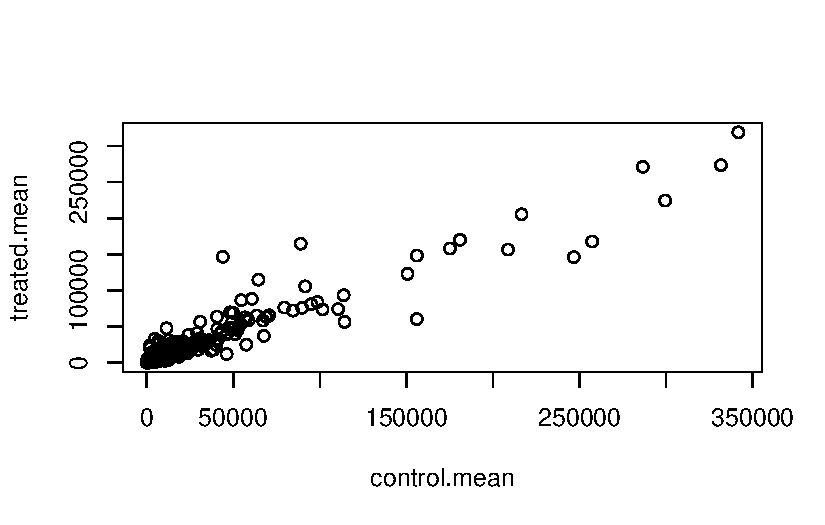
\includegraphics[keepaspectratio]{Class13_files/figure-pdf/unnamed-chunk-7-1.pdf}}

Our count data is highly skewed and when we see a pattern like this plot
it SCREEMS log transform me

\begin{Shaded}
\begin{Highlighting}[]
\FunctionTok{plot}\NormalTok{(meancounts, }\AttributeTok{log =} \StringTok{"xy"}\NormalTok{)}
\end{Highlighting}
\end{Shaded}

\begin{verbatim}
Warning in xy.coords(x, y, xlabel, ylabel, log): 15032 x values <= 0 omitted
from logarithmic plot
\end{verbatim}

\begin{verbatim}
Warning in xy.coords(x, y, xlabel, ylabel, log): 15281 y values <= 0 omitted
from logarithmic plot
\end{verbatim}

\pandocbounded{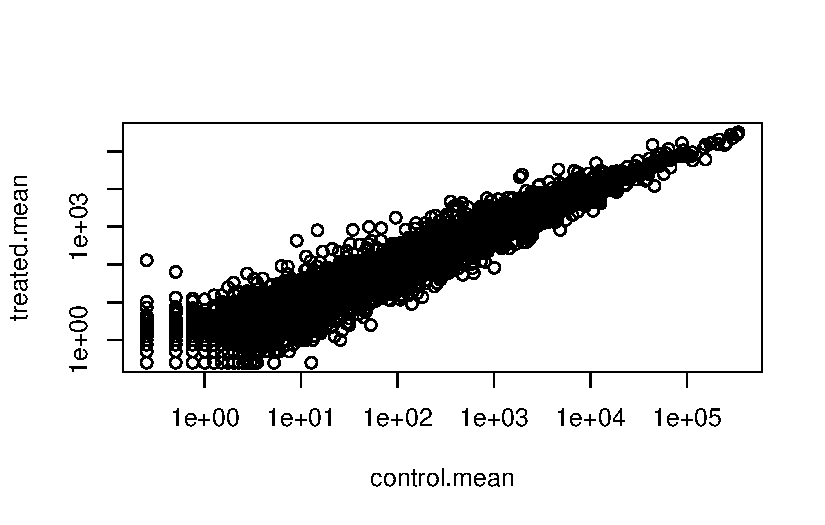
\includegraphics[keepaspectratio]{Class13_files/figure-pdf/unnamed-chunk-8-1.pdf}}

We often use log2 transform for this kind of data in bioinformatics
because it makes my brain hurt less

\begin{Shaded}
\begin{Highlighting}[]
\CommentTok{\# Treated / Control}

\FunctionTok{log2}\NormalTok{(}\DecValTok{20}\SpecialCharTok{/}\DecValTok{20}\NormalTok{)}
\end{Highlighting}
\end{Shaded}

\begin{verbatim}
[1] 0
\end{verbatim}

\begin{Shaded}
\begin{Highlighting}[]
\FunctionTok{log2}\NormalTok{(}\DecValTok{40}\SpecialCharTok{/}\DecValTok{20}\NormalTok{)}
\end{Highlighting}
\end{Shaded}

\begin{verbatim}
[1] 1
\end{verbatim}

\begin{Shaded}
\begin{Highlighting}[]
\FunctionTok{log2}\NormalTok{(}\DecValTok{20}\SpecialCharTok{/}\DecValTok{40}\NormalTok{)}
\end{Highlighting}
\end{Shaded}

\begin{verbatim}
[1] -1
\end{verbatim}

\begin{Shaded}
\begin{Highlighting}[]
\FunctionTok{log2}\NormalTok{(}\DecValTok{80}\SpecialCharTok{/}\DecValTok{20}\NormalTok{)}
\end{Highlighting}
\end{Shaded}

\begin{verbatim}
[1] 2
\end{verbatim}

We call this little fraction the \textbf{``log2 fold change''} as it
tells us how much mroe or less gene expression we have in units of
doubling, etc.

Let's calculate the log2 fold change for our `treated.mean' and
`control.mean' counts and call this `log2fc'.

\begin{Shaded}
\begin{Highlighting}[]
\NormalTok{meancounts}\SpecialCharTok{$}\NormalTok{log2fc }\OtherTok{\textless{}{-}} \FunctionTok{log2}\NormalTok{( meancounts}\SpecialCharTok{$}\NormalTok{treated.mean }\SpecialCharTok{/} 
\NormalTok{                             meancounts}\SpecialCharTok{$}\NormalTok{control.mean )}
\FunctionTok{head}\NormalTok{(meancounts)}
\end{Highlighting}
\end{Shaded}

\begin{verbatim}
                control.mean treated.mean      log2fc
ENSG00000000003       900.75       658.00 -0.45303916
ENSG00000000005         0.00         0.00         NaN
ENSG00000000419       520.50       546.00  0.06900279
ENSG00000000457       339.75       316.50 -0.10226805
ENSG00000000460        97.25        78.75 -0.30441833
ENSG00000000938         0.75         0.00        -Inf
\end{verbatim}

A common ``rule of thumb'' threshold for calling a gene ``up regulated''
or ``down regulated'' is a log2 fold chnage value of +2 or -2 (or
greater)

\subsection{DESeq Analysis}\label{deseq-analysis}

Let's do this analysis properly and not forget about the significance of
the differences.

For this we will use the \textbf{DESeq2} package

\begin{Shaded}
\begin{Highlighting}[]
\FunctionTok{library}\NormalTok{(DESeq2)}
\end{Highlighting}
\end{Shaded}

To run a DESeq analysis we need at least two inputs:

\begin{itemize}
\tightlist
\item
  `countData' i.e.~are gene counts across different experiements
\item
  `colData' i.e.~our metadata about those count columns
\end{itemize}

\begin{Shaded}
\begin{Highlighting}[]
\NormalTok{dds }\OtherTok{\textless{}{-}} \FunctionTok{DESeqDataSetFromMatrix}\NormalTok{(}\AttributeTok{countData =}\NormalTok{ counts,}
                              \AttributeTok{colData =}\NormalTok{ metadata,}
                              \AttributeTok{design =} \SpecialCharTok{\textasciitilde{}}\NormalTok{dex)}
\end{Highlighting}
\end{Shaded}

\begin{verbatim}
converting counts to integer mode
\end{verbatim}

Now we can run the DESeq analysis pipeline using this `dds' object that
has all the inputs we need.

\begin{Shaded}
\begin{Highlighting}[]
\NormalTok{dds}\OtherTok{\textless{}{-}} \FunctionTok{DESeq}\NormalTok{(dds)}
\end{Highlighting}
\end{Shaded}

\begin{verbatim}
estimating size factors
\end{verbatim}

\begin{verbatim}
estimating dispersions
\end{verbatim}

\begin{verbatim}
gene-wise dispersion estimates
\end{verbatim}

\begin{verbatim}
mean-dispersion relationship
\end{verbatim}

\begin{verbatim}
final dispersion estimates
\end{verbatim}

\begin{verbatim}
fitting model and testing
\end{verbatim}

\begin{Shaded}
\begin{Highlighting}[]
\NormalTok{res }\OtherTok{\textless{}{-}} \FunctionTok{results}\NormalTok{(dds)}
\FunctionTok{head}\NormalTok{(res)}
\end{Highlighting}
\end{Shaded}

\begin{verbatim}
log2 fold change (MLE): dex treated vs control 
Wald test p-value: dex treated vs control 
DataFrame with 6 rows and 6 columns
                  baseMean log2FoldChange     lfcSE      stat    pvalue
                 <numeric>      <numeric> <numeric> <numeric> <numeric>
ENSG00000000003 747.194195      -0.350703  0.168242 -2.084514 0.0371134
ENSG00000000005   0.000000             NA        NA        NA        NA
ENSG00000000419 520.134160       0.206107  0.101042  2.039828 0.0413675
ENSG00000000457 322.664844       0.024527  0.145134  0.168996 0.8658000
ENSG00000000460  87.682625      -0.147143  0.256995 -0.572550 0.5669497
ENSG00000000938   0.319167      -1.732289  3.493601 -0.495846 0.6200029
                     padj
                <numeric>
ENSG00000000003  0.163017
ENSG00000000005        NA
ENSG00000000419  0.175937
ENSG00000000457  0.961682
ENSG00000000460  0.815805
ENSG00000000938        NA
\end{verbatim}

\subsection{Volcano Plot}\label{volcano-plot}

This is a ubiquitous and common visulaization for this type of data that
puts the log2 fold change and the adjusted p-value together in one plot
that poeple can get insight for what is going on in the whole dataset
results.

\begin{Shaded}
\begin{Highlighting}[]
\FunctionTok{library}\NormalTok{(ggplot2)}
\end{Highlighting}
\end{Shaded}

\begin{Shaded}
\begin{Highlighting}[]
\FunctionTok{ggplot}\NormalTok{(res) }\SpecialCharTok{+}
  \FunctionTok{aes}\NormalTok{(}\AttributeTok{x =}\NormalTok{ log2FoldChange, }\AttributeTok{y =}\NormalTok{ padj) }\SpecialCharTok{+}
  \FunctionTok{geom\_point}\NormalTok{(}\AttributeTok{alpha=}\FloatTok{0.3}\NormalTok{)}
\end{Highlighting}
\end{Shaded}

\begin{verbatim}
Warning: Removed 23549 rows containing missing values or values outside the scale range
(`geom_point()`).
\end{verbatim}

\pandocbounded{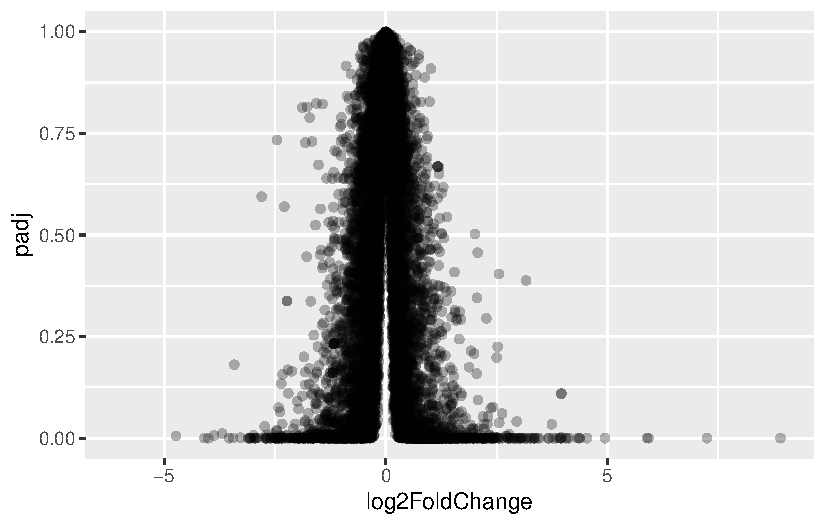
\includegraphics[keepaspectratio]{Class13_files/figure-pdf/unnamed-chunk-15-1.pdf}}

That plot is not very useful because we don't care about genes with high
p-values, we want the very low values below our alpha threshold
(e.g.~0.01)

Let's log the y-axis so we can see these gene/points moreclearly:

\begin{Shaded}
\begin{Highlighting}[]
\FunctionTok{ggplot}\NormalTok{(res) }\SpecialCharTok{+}
  \FunctionTok{aes}\NormalTok{(log2FoldChange, }\FunctionTok{log}\NormalTok{(padj)) }\SpecialCharTok{+}
  \FunctionTok{geom\_point}\NormalTok{()}
\end{Highlighting}
\end{Shaded}

\begin{verbatim}
Warning: Removed 23549 rows containing missing values or values outside the scale range
(`geom_point()`).
\end{verbatim}

\pandocbounded{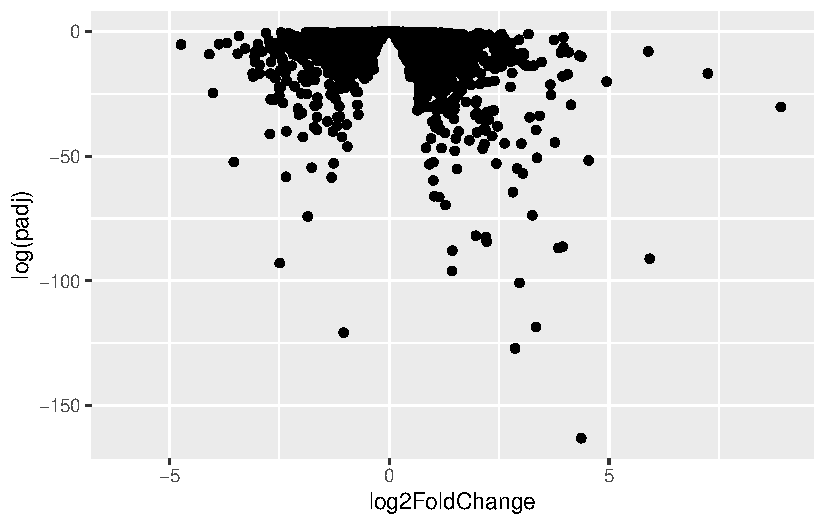
\includegraphics[keepaspectratio]{Class13_files/figure-pdf/unnamed-chunk-16-1.pdf}}

We need to flip the y-axis for our ``volcano''

\begin{Shaded}
\begin{Highlighting}[]
\FunctionTok{ggplot}\NormalTok{(res) }\SpecialCharTok{+}
  \FunctionTok{aes}\NormalTok{(log2FoldChange, }\SpecialCharTok{{-}}\FunctionTok{log}\NormalTok{(padj)) }\SpecialCharTok{+}
  \FunctionTok{geom\_point}\NormalTok{()}
\end{Highlighting}
\end{Shaded}

\begin{verbatim}
Warning: Removed 23549 rows containing missing values or values outside the scale range
(`geom_point()`).
\end{verbatim}

\pandocbounded{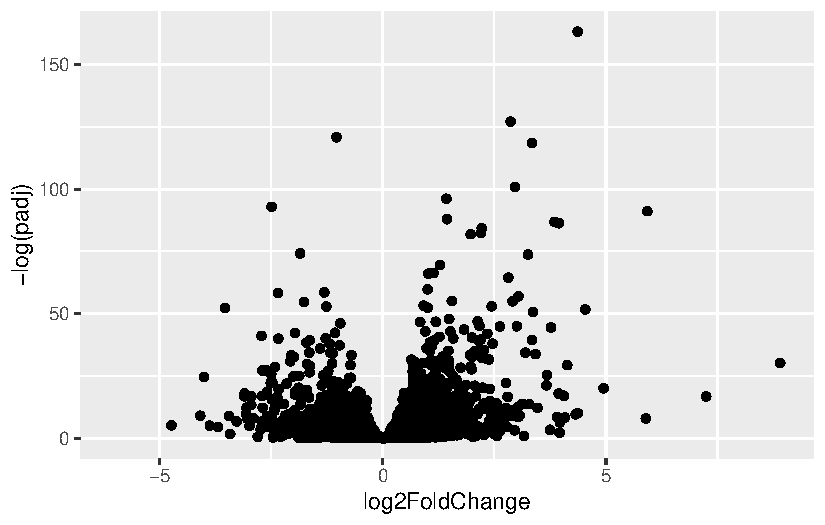
\includegraphics[keepaspectratio]{Class13_files/figure-pdf/unnamed-chunk-17-1.pdf}}

\begin{quote}
Q. Add annotation to this volcano plot including the log2 fold-change
threshold of +2 and -2 and the p-value threshold of 0.05. Also color up
just the genes that meet both these thresholds. These are the ones we
will focus on next day!
\end{quote}

\subsection{Save Our Results}\label{save-our-results}

\begin{Shaded}
\begin{Highlighting}[]
\FunctionTok{write.csv}\NormalTok{(res, }\AttributeTok{file =} \StringTok{"myresults.csv"}\NormalTok{)}
\end{Highlighting}
\end{Shaded}

\subsection{Add annotation data}\label{add-annotation-data}

We need to ``map or''translate'' out ENSEN+MBLE gene identifiers in out
results object to date to the identifiers used in different databases we
want to use for learning more about these

For this we will use a couple of Bioconductor packages that we can
install with: BiocManager:: install''AnnotationDbi'') and BiocManager::
install(``org.Hs.eg.db'')

\begin{Shaded}
\begin{Highlighting}[]
\FunctionTok{library}\NormalTok{(}\StringTok{"AnnotationDbi"}\NormalTok{)}
\FunctionTok{library}\NormalTok{(}\StringTok{"org.Hs.eg.db"}\NormalTok{)}
\end{Highlighting}
\end{Shaded}

We can see the columns in org.HS

We can now use the `mapsIDs()' function to map between these different
database identifier formats:

\begin{Shaded}
\begin{Highlighting}[]
\NormalTok{res}\SpecialCharTok{$}\NormalTok{symbol }\OtherTok{\textless{}{-}} \FunctionTok{mapIds}\NormalTok{(org.Hs.eg.db,}
                     \AttributeTok{keys =} \FunctionTok{row.names}\NormalTok{(res),}
                     \AttributeTok{keytype =} \StringTok{"ENSEMBL"}\NormalTok{,}
                     \AttributeTok{column =} \StringTok{"SYMBOL"}\NormalTok{)}
\end{Highlighting}
\end{Shaded}

\begin{verbatim}
'select()' returned 1:many mapping between keys and columns
\end{verbatim}

\subsection{Pathway Analysis}\label{pathway-analysis}

Now we ave our annotated results with their log2 fold change and p
values we can figure out which biological pathways and processes these
genes are involved with.

We will use the \textbf{gage} and \textbf{pathview} packages fir tgus
steo and we can install them with: BiocManager::install( c(``pathview'',
``gage'', ``gageData'') )

\begin{Shaded}
\begin{Highlighting}[]
\FunctionTok{library}\NormalTok{(gage)}
\FunctionTok{library}\NormalTok{(gageData)}
\FunctionTok{library}\NormalTok{(pathview)}
\end{Highlighting}
\end{Shaded}

Let's have a wee peak at the gageData

\begin{Shaded}
\begin{Highlighting}[]
\FunctionTok{data}\NormalTok{(kegg.sets.hs)}
\FunctionTok{head}\NormalTok{(kegg.sets.hs, }\DecValTok{2}\NormalTok{)}
\end{Highlighting}
\end{Shaded}

\begin{verbatim}
$`hsa00232 Caffeine metabolism`
[1] "10"   "1544" "1548" "1549" "1553" "7498" "9"   

$`hsa00983 Drug metabolism - other enzymes`
 [1] "10"     "1066"   "10720"  "10941"  "151531" "1548"   "1549"   "1551"  
 [9] "1553"   "1576"   "1577"   "1806"   "1807"   "1890"   "221223" "2990"  
[17] "3251"   "3614"   "3615"   "3704"   "51733"  "54490"  "54575"  "54576" 
[25] "54577"  "54578"  "54579"  "54600"  "54657"  "54658"  "54659"  "54963" 
[33] "574537" "64816"  "7083"   "7084"   "7172"   "7363"   "7364"   "7365"  
[41] "7366"   "7367"   "7371"   "7372"   "7378"   "7498"   "79799"  "83549" 
[49] "8824"   "8833"   "9"      "978"   
\end{verbatim}

We need a named vector oof importance (e.g.~fold change values) that has
gene ids as names. These names need to be in the correct format (using
the correct database format for the ids).

\begin{Shaded}
\begin{Highlighting}[]
\NormalTok{x }\OtherTok{\textless{}{-}} \FunctionTok{c}\NormalTok{(}\DecValTok{10}\NormalTok{, }\DecValTok{9}\NormalTok{, }\DecValTok{7}\NormalTok{)}
\FunctionTok{names}\NormalTok{(x) }\OtherTok{\textless{}{-}} \FunctionTok{c}\NormalTok{(}\StringTok{"alice"}\NormalTok{, }\StringTok{"chandea"}\NormalTok{, }\StringTok{"barry"}\NormalTok{)}
\NormalTok{x}
\end{Highlighting}
\end{Shaded}

\begin{verbatim}
  alice chandea   barry 
     10       9       7 
\end{verbatim}

\begin{Shaded}
\begin{Highlighting}[]
\FunctionTok{names}\NormalTok{(x)}
\end{Highlighting}
\end{Shaded}

\begin{verbatim}
[1] "alice"   "chandea" "barry"  
\end{verbatim}

Here we will make a wee inout vector called `foldchanges' that has
`entrez' ids as well as names.

\begin{Shaded}
\begin{Highlighting}[]
\NormalTok{foldchanges }\OtherTok{\textless{}{-}}\NormalTok{ res}\SpecialCharTok{$}\NormalTok{log2FoldChange}
\FunctionTok{names}\NormalTok{(foldchanges) }\OtherTok{\textless{}{-}}\NormalTok{ res}\SpecialCharTok{$}\NormalTok{entrez}
\end{Highlighting}
\end{Shaded}

Now we can run `gage()' to do our pathway analysis.

\begin{Shaded}
\begin{Highlighting}[]
\NormalTok{keggres }\OtherTok{=} \FunctionTok{gage}\NormalTok{(foldchanges, }\AttributeTok{gsets=}\NormalTok{kegg.sets.hs)}
\end{Highlighting}
\end{Shaded}

\begin{Shaded}
\begin{Highlighting}[]
\FunctionTok{attributes}\NormalTok{(keggres)}
\end{Highlighting}
\end{Shaded}

\begin{verbatim}
$names
[1] "greater" "less"    "stats"  
\end{verbatim}

The top 3 overlapping pathways from KEGG

\begin{Shaded}
\begin{Highlighting}[]
\FunctionTok{head}\NormalTok{(keggres}\SpecialCharTok{$}\NormalTok{less, }\DecValTok{3}\NormalTok{)}
\end{Highlighting}
\end{Shaded}

\begin{verbatim}
                                         p.geomean stat.mean p.val q.val
hsa00232 Caffeine metabolism                    NA       NaN    NA    NA
hsa00983 Drug metabolism - other enzymes        NA       NaN    NA    NA
hsa01100 Metabolic pathways                     NA       NaN    NA    NA
                                         set.size exp1
hsa00232 Caffeine metabolism                    0   NA
hsa00983 Drug metabolism - other enzymes        0   NA
hsa01100 Metabolic pathways                     0   NA
\end{verbatim}

Now we can use the \textbf{pathview} package with the found KEGG pathway
IDs (e.g.~``hsa05310 for the Asthma pathway) to make a pathway figure
showing our Differential Expressed Genes (DSGs)

\begin{Shaded}
\begin{Highlighting}[]
\FunctionTok{pathview}\NormalTok{(}\AttributeTok{gene.data=}\NormalTok{foldchanges, }\AttributeTok{pathway.id=}\StringTok{"hsa05310"}\NormalTok{)}
\end{Highlighting}
\end{Shaded}

\begin{verbatim}
Warning: None of the genes or compounds mapped to the pathway!
Argument gene.idtype or cpd.idtype may be wrong.
\end{verbatim}

\begin{verbatim}
'select()' returned 1:1 mapping between keys and columns
\end{verbatim}

\begin{verbatim}
Info: Working in directory /Users/yassi/Desktop/BIMM143/Class13
\end{verbatim}

\begin{verbatim}
Info: Writing image file hsa05310.pathview.png
\end{verbatim}

\pandocbounded{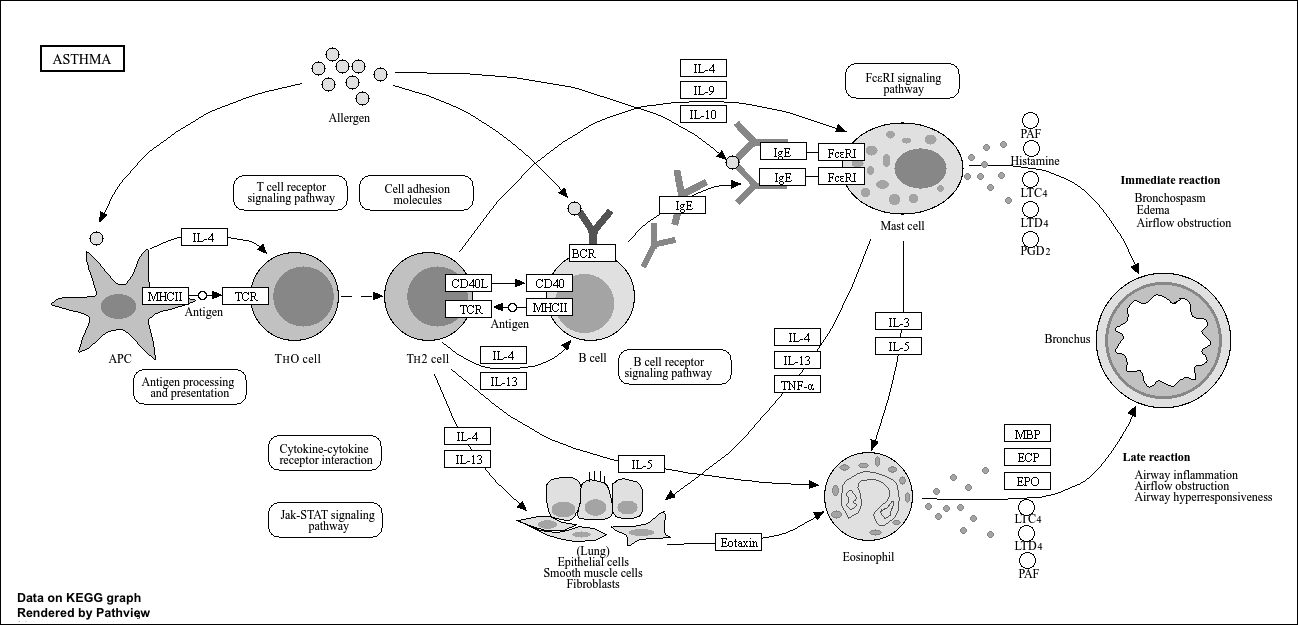
\includegraphics[keepaspectratio]{hsa05310.pathview.png}}

\subsection{Save out annoted results}\label{save-out-annoted-results}

\begin{Shaded}
\begin{Highlighting}[]
\FunctionTok{write.csv}\NormalTok{(res, }\AttributeTok{file=}\StringTok{"myresults\_annotated.csv"}\NormalTok{)}
\end{Highlighting}
\end{Shaded}





\end{document}
